\documentclass[11pt,letterpaper]{article}
\usepackage[utf8]{inputenc}
\usepackage[top=2.54cm,bottom=2.54cm,left=4cm,right=2.5cm,headheight=14pt]{geometry}
\usepackage{graphicx}
\usepackage[hidelinks,bookmarksnumbered]{hyperref}
\usepackage[all]{hypcap}
\usepackage{fancyhdr}
\usepackage[calcwidth]{titlesec}
\usepackage{chngcntr}
\usepackage{bytefield}
\usepackage{booktabs}
\usepackage[x11names]{xcolor}
\usepackage{listings}
\usepackage[section]{placeins}
\usepackage[style=iso]{datetime2}
\usepackage{pgf-umlsd}
\usepackage{amsmath}
\usepackage{cite}
\usepackage[nottoc,numbib]{tocbibind}
\usepackage{colortbl}
\usepackage{caption}
\usepackage{textcomp}
\usepackage{listings}
\usepackage{longtable}
\usepackage{minted}
\usepackage[nobreak=true]{mdframed}

\surroundwithmdframed{minted}
\surroundwithmdframed{verbatim}

\DeclareCaptionFont{blue}{\color{LightSteelBlue3}}
\newcommand{\foo}{\color{LightSteelBlue3}\makebox[0pt]{\textbullet}\hskip-0.5pt\vrule width 1pt\hspace{\labelsep}}

\let\Oldsection\section
\renewcommand{\section}{\FloatBarrier\Oldsection}

\let\Oldsubsection\subsection
\renewcommand{\subsection}{\FloatBarrier\Oldsubsection}

\let\Oldsubsubsection\subsubsection
\renewcommand{\subsubsection}{\FloatBarrier\Oldsubsubsection}

\title{L3-T-2 Design Document}
\author{Samuel Dewan, Sunjeevani Pujari, Mario Shebib and Morgan Smith}

% Headers and footers
\pagestyle{fancy}
\fancyhf{}
\lhead{SYSC3010 Project Design Document}
\rhead{Group L3-T-2}
\rfoot{\thepage}

% More space around figures
\setlength\intextsep{18pt}
% Per section figure and table numbers
\counterwithin{figure}{section}
\counterwithin{table}{section}

% Colour links rather than putting a box around them
\hypersetup{
    colorlinks,
    linkcolor={black},
    citecolor={blue!50!black},
    urlcolor={blue!80!black},
}

% More space between table rows
\renewcommand{\arraystretch}{1.2}

% Section numbers in the margin
\newcommand{\marginsecnumber}[1]{%
    \makebox[0pt][r]{#1\hspace{6pt}}%
}
\titleformat{\section}
    {\sffamily\Large\bfseries}
    {\marginsecnumber\thesection}
    {0pt}
    {}
\titleformat{\subsection}
    {\sffamily\large\bfseries}
    {\marginsecnumber\thesubsection}
    {0pt}
    {}
\titleformat{\subsubsection}
    {\sffamily\normalsize\bfseries}
    {\marginsecnumber\thesubsubsection}
    {0pt}
    {}

% Draft watermark
\usepackage{eso-pic,graphicx}
\AddToShipoutPicture*{%
    \AtTextCenter{%
        \makebox(0,0)[c]{\resizebox{\textwidth}{!}{%
        \rotatebox{45}{\textsf{\textbf{\color{lightgray}DRAFT}}}}}
    }
}

\begin{document}
\frenchspacing

\pagenumbering{Alph}
\begin{titlepage}
\centering

\vspace*{\stretch{2}}

{\Huge \sffamily Project Design Document}

\vspace{\stretch{1}}
{\large \textbf{SYSC3010}}

{\large \textbf{Fall 2020}}

Prof. Cheryl Schramm

\vspace{\stretch{2}}

{\large \textbf{Group L3-T-2}}

Samuel Dewan

{\footnotesize samueldewan@cmail.carleton.ca}

Sunjeevani Pujari

{\footnotesize sunjeevanipujari@cmail.carleton.ca}

Mario Shebib

{\footnotesize marioshebib@cmail.carleton.ca}

Morgan Smith

{\footnotesize morgansmith@cmail.carleton.ca}

\vspace{\stretch{2}}

{\large \today}

\vspace{\stretch{3}}

\end{titlepage}

\pagenumbering{Roman}
\tableofcontents
\clearpage
\pagenumbering{arabic}

\section{Problem Statement}
\label{sec:problem-statement}
Our access control system will be designed to meet the needs of employers to
look after the safety of their employees. The scope of this project is to
provide employers with an access control system that grants access to employees
entering the workplace based on their measured body temperature. As studies
show that fever is the most frequent symptom in more than 50\% of COVID-19
cases our system also blocks access to employees with a body temperature
indicating a fever for 14 days to prevent the spread of COVID-19 in the
workplace. Additionally, our system helps building owners adhere to social
distancing guidelines implemented by the government by keeping track of the
number of people on the premises and restricts employees from entering the
building when the maximum threshold for the workplace has been
attained. Although not in the scope of the project, our system would work with
employers to comply with their standards and constraints to provide their
employees access to a COVID-19 free workplace. Our system aims to enable a
COVID-19 free work environment.

Our access control system is a technology-based solution using a data collection
and management system whose primary features and their functionalities include:

\todo{Clean up the list. Maybe don't have control server under control
server. Also remove points of being available at each entry way}

\subsection{Door Node}
\begin{itemize}
    \item NFC security badge reader
    \begin{itemize}
        \item Available at each door node at both entry and exit ways
        \item Read valid NFC card ID and associate with employee ID
    \end{itemize}
    \item Infrared temperature sensor
    \begin{itemize}
        \item Available at each entry way
        \item Measure the body temperature of an employee trying to enter the
              work premises
        \item Alert control server in case of high temperature reading
    \end{itemize}
    \item Time of flight distance sensor
    \begin{itemize}
        \item Available at each entry way
        \item Identify if the employee is standing at an ideal distance from the
              temperature sensor.
    \end{itemize}
    \item LED display
    \begin{itemize}
        \item Available at each entry way
        \item Display a green light at the entrance if accepting employee entry
        \item Display a red circle light at the entrance when control server
              restricts access due to premises acquiring maximum threshold
        \item Display orange light if employee in range of the temperature
              sensor
        \item Display red light if employee not in range of temperature sensor
        \item Display flashing green light if control server authorizes employee
              to access after having temperature recorded
        \item Display flashing red light if control server unauthorizes employee
              from accessing the building after having temperature recorded 
    \end{itemize}
    \item Electronic door lock
    \begin{itemize}
        \item Available at each door node at both entry and exit ways
        \item Unlock only when control server authorizes the employee to
              enter/exit premises
        \item Locked when control server prevents access to employees with
              recorded fever temperatures
        \item Locked at entry ways when control server restricts access due to
              premises acquiring maximum threshold
    \end{itemize}
\end{itemize}

\subsection{Control server}

\begin{itemize}
    \item Control server
    \begin{itemize}
        \item Able to access all door nodes
        \item Able to access database and available tables
        \item Identifies number of people entering and exiting the premises
        \item Initializes access restriction when maximum threshold of premises
              is acquired
    \end{itemize}
    \item Database
    \begin{itemize}
        \item Properly organized tables with appropriate entries for each
              individual field
        \item Properly formatted values for sensor recorded data fields
        \item Records of the temperature readings of all employees are
              accessible for at least 14 days 
    \end{itemize}
    \item Operator GUI
    \begin{itemize}
        \item Able to add new employee information
        \item Able to view details of all employees based on NFC security card
              user id and employee id
        \item Able to approve quarantine period initiated by the control server
              for individual employees
    \end{itemize}
\end{itemize}


\clearpage

\section{Design Overview}
\label{sec:design-overview}
\subsection{Architecture}

Our product it made up of two parts: the control server, and the door nodes.
Our product interacts with two types of actors: Operators and Users.

The control server maintains a database of operator profiles, operator logs,
user profiles, and interaction logs.  The control server will use the operator
profiles to validate users using the operator GUI.  Every action performed in
the operator GUI will be logged in the operator logs.  Operators can create and
modify user profiles.  When a user attempts to use a door node, their identity
is checked against their user profile.  Each interaction with a door node is
recorded in a user log.

\begin{figure}[!htb]
\centering
\includegraphics[width=\textwidth]{figures/architecture.png}
\caption{UML Architecture Diagram}
\label{fig:architecture-diagram}
\end{figure}

\subsection{Communication Protocol}

\begin{itemize}
\item Account ID: (number) uniquely identifies an account
\item Node ID: (number) uniquely identifies a door node
\item Transaction ID: (number) uniquely identifies a transaction
\item Current time: (number) Time message was sent
\item Information Request: (list of keys) A list of information required to further the
transaction
\item Information Response: (list of key value pairs) Contains obtained information
\item Access Request Response: (boolean)
\end{itemize}

\begin{table*}[htb]
\begin{tabular}{ l | l | l | p{4.5cm} }
\toprule
Sender & Receiver & Message & Data Format\\
\midrule
Door Node & Control Server & ACCESS\_REQUEST &
Node ID \newline Transaction ID \newline Current time \newline Account ID\\
\hline
Door Node & Control Server & INFORMATION\_RESPONSE &
Node ID \newline Transaction ID \newline Current time \newline Information Response\\
\hline
Control Server & Door Node & INFORMATION\_REQUEST &
Node ID \newline Transaction ID \newline Current time \newline Information Request\\
\hline
Control Server & Door Node & ACCESS\_RESPONSE &
Node ID \newline Transaction ID \newline Current time \newline Account ID \newline Access Request Response\\
\bottomrule
\end{tabular}
\caption{Messages}
\end{table*}

\subsection{Message Sequence Diagrams}

\begin{figure}[!htb]
\centering
\includegraphics[width=\textwidth]{figures/message-sequence-diagram.png}
\caption{Message Sequence Diagram}
\label{fig:message-sequence-diagram}
\end{figure}

\subsection{Database Schema}

\begin{figure}[!htb]
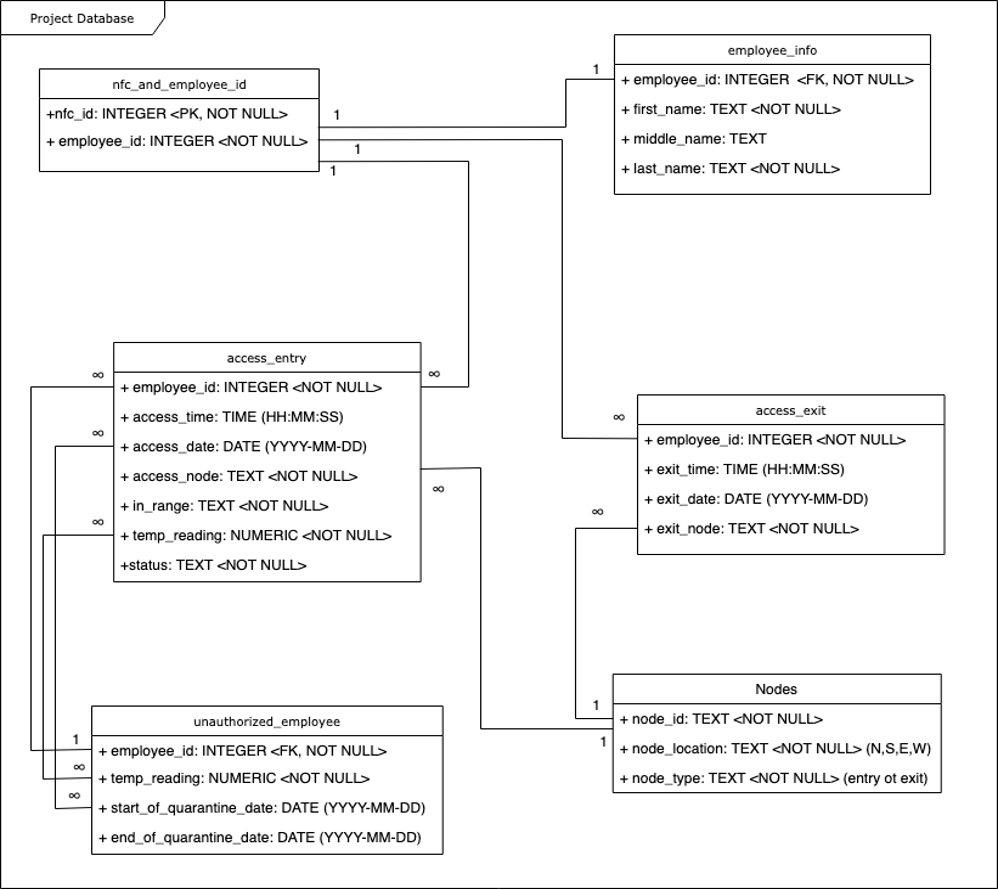
\includegraphics[width=\textwidth]{figures/db-schema.png}
\caption{Database Schema}
\end{figure}


\clearpage

\section{Software Design}
\label{sec:software-design}
\subsection{Class Diagram}

\begin{figure}[!htb]
\centering
\includegraphics[width=\textwidth]{uml/class-diagram.png}
\caption{Class Diagram}
\label{fig:class-diagram}
\end{figure}

\subsection{Door Node}

\begin{figure}[!htb]
\centering
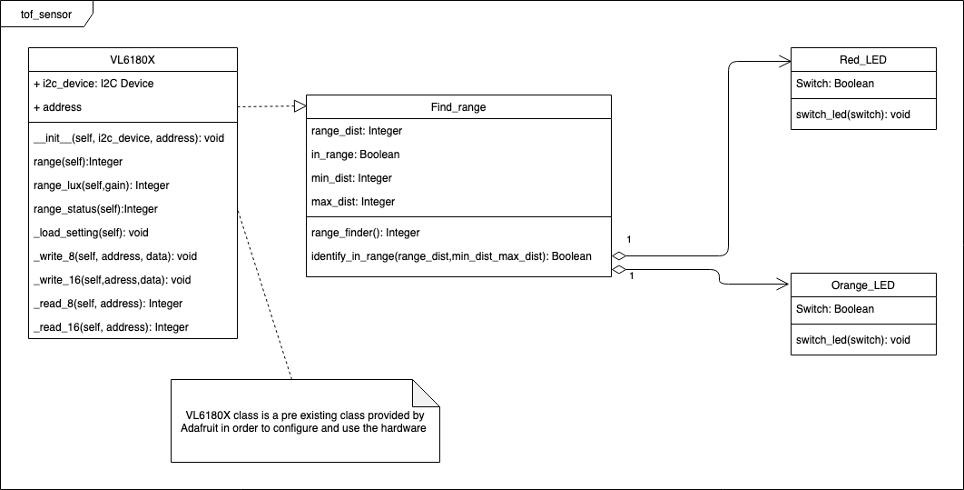
\includegraphics[width=\textwidth]{images/tof-driver-class-dia.png}
\caption{Class Diagram for Time of Flight Range Sensor Driver}
\end{figure}

\begin{figure}[!htb]
\centering
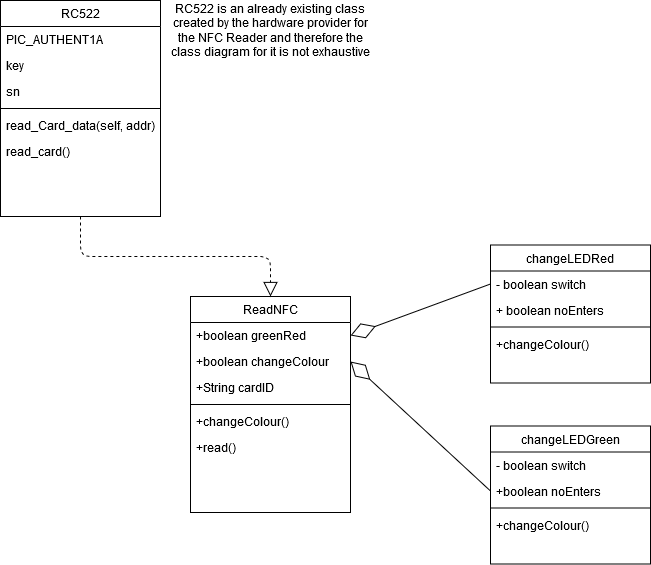
\includegraphics[width=\textwidth]{images/nfc-driver-class-dia.png}
\caption{Class Diagram for NFC Security Badge Reader Driver}
\end{figure}

\begin{figure}[!htb]
\centering
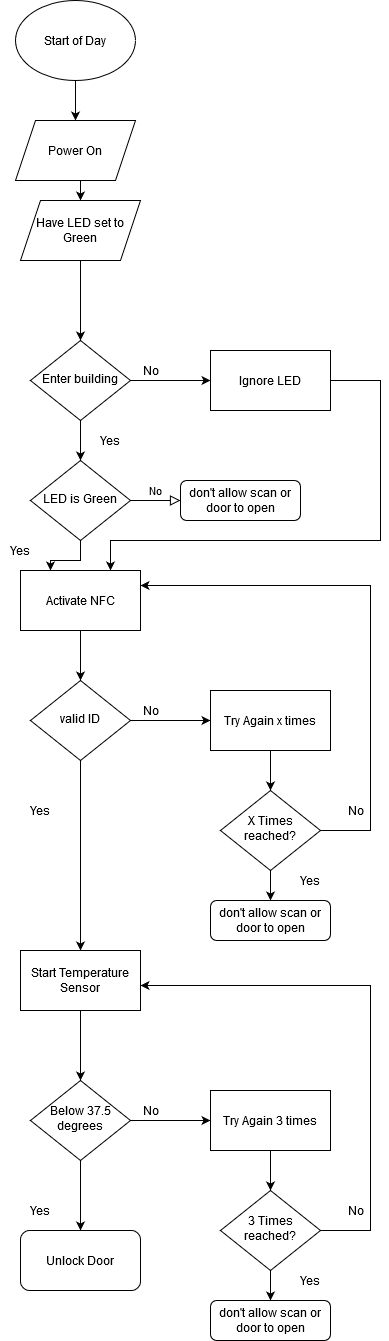
\includegraphics[width=0.4\textwidth]{images/door-interface-flow.png}
\caption{Flow of Door Node Software}
\end{figure}

\subsection{Control Server}

\begin{figure}[!htb]
\centering
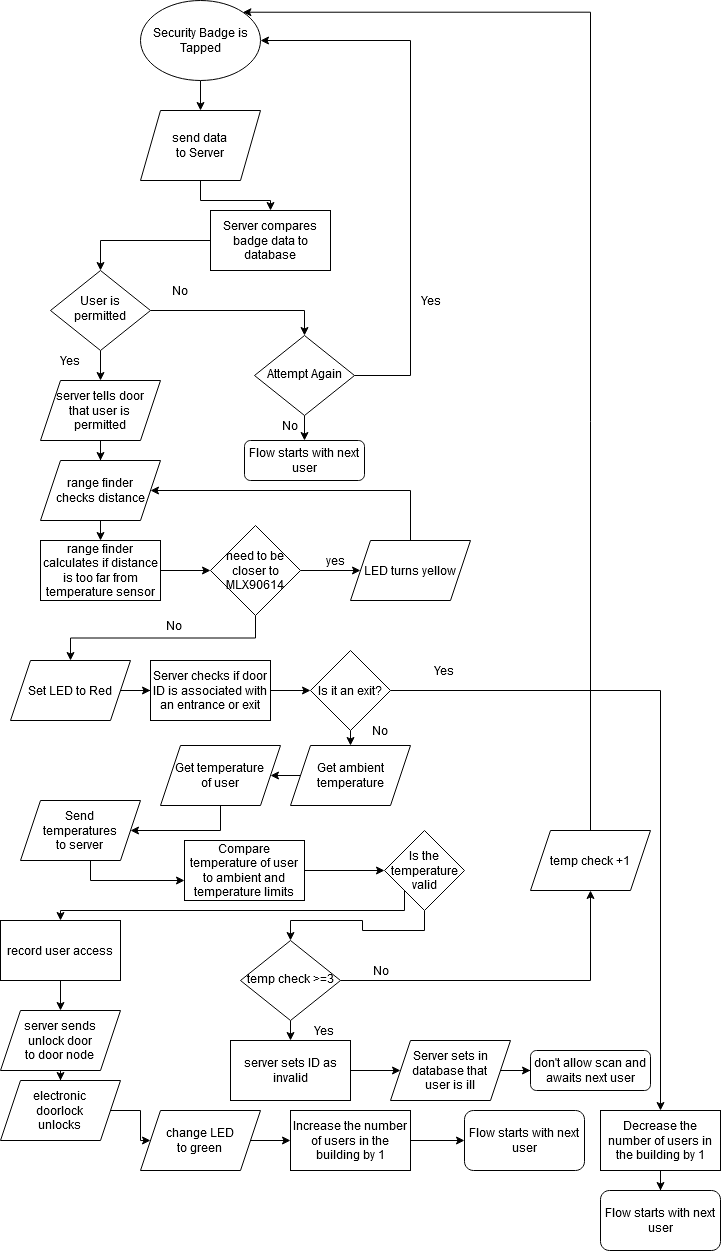
\includegraphics[width=0.5\textwidth]{images/server-door-msg-flow.png}
\caption{Flow of Communication Between Control Server and Door Node}
\end{figure}



\clearpage

\section{Hardware Design}
\label{sec:hardware-design}
The door node is the hardware that will be located at each door. It consists of
a NFC security badge reader, infrared temperature sensor, time of flight range
sensor and electronic door lock, all connected to a Raspberry Pi.

Figure \ref{fig:door-node-schematic} shows a schematic of the door node.

\begin{figure}[!htb]
\centering
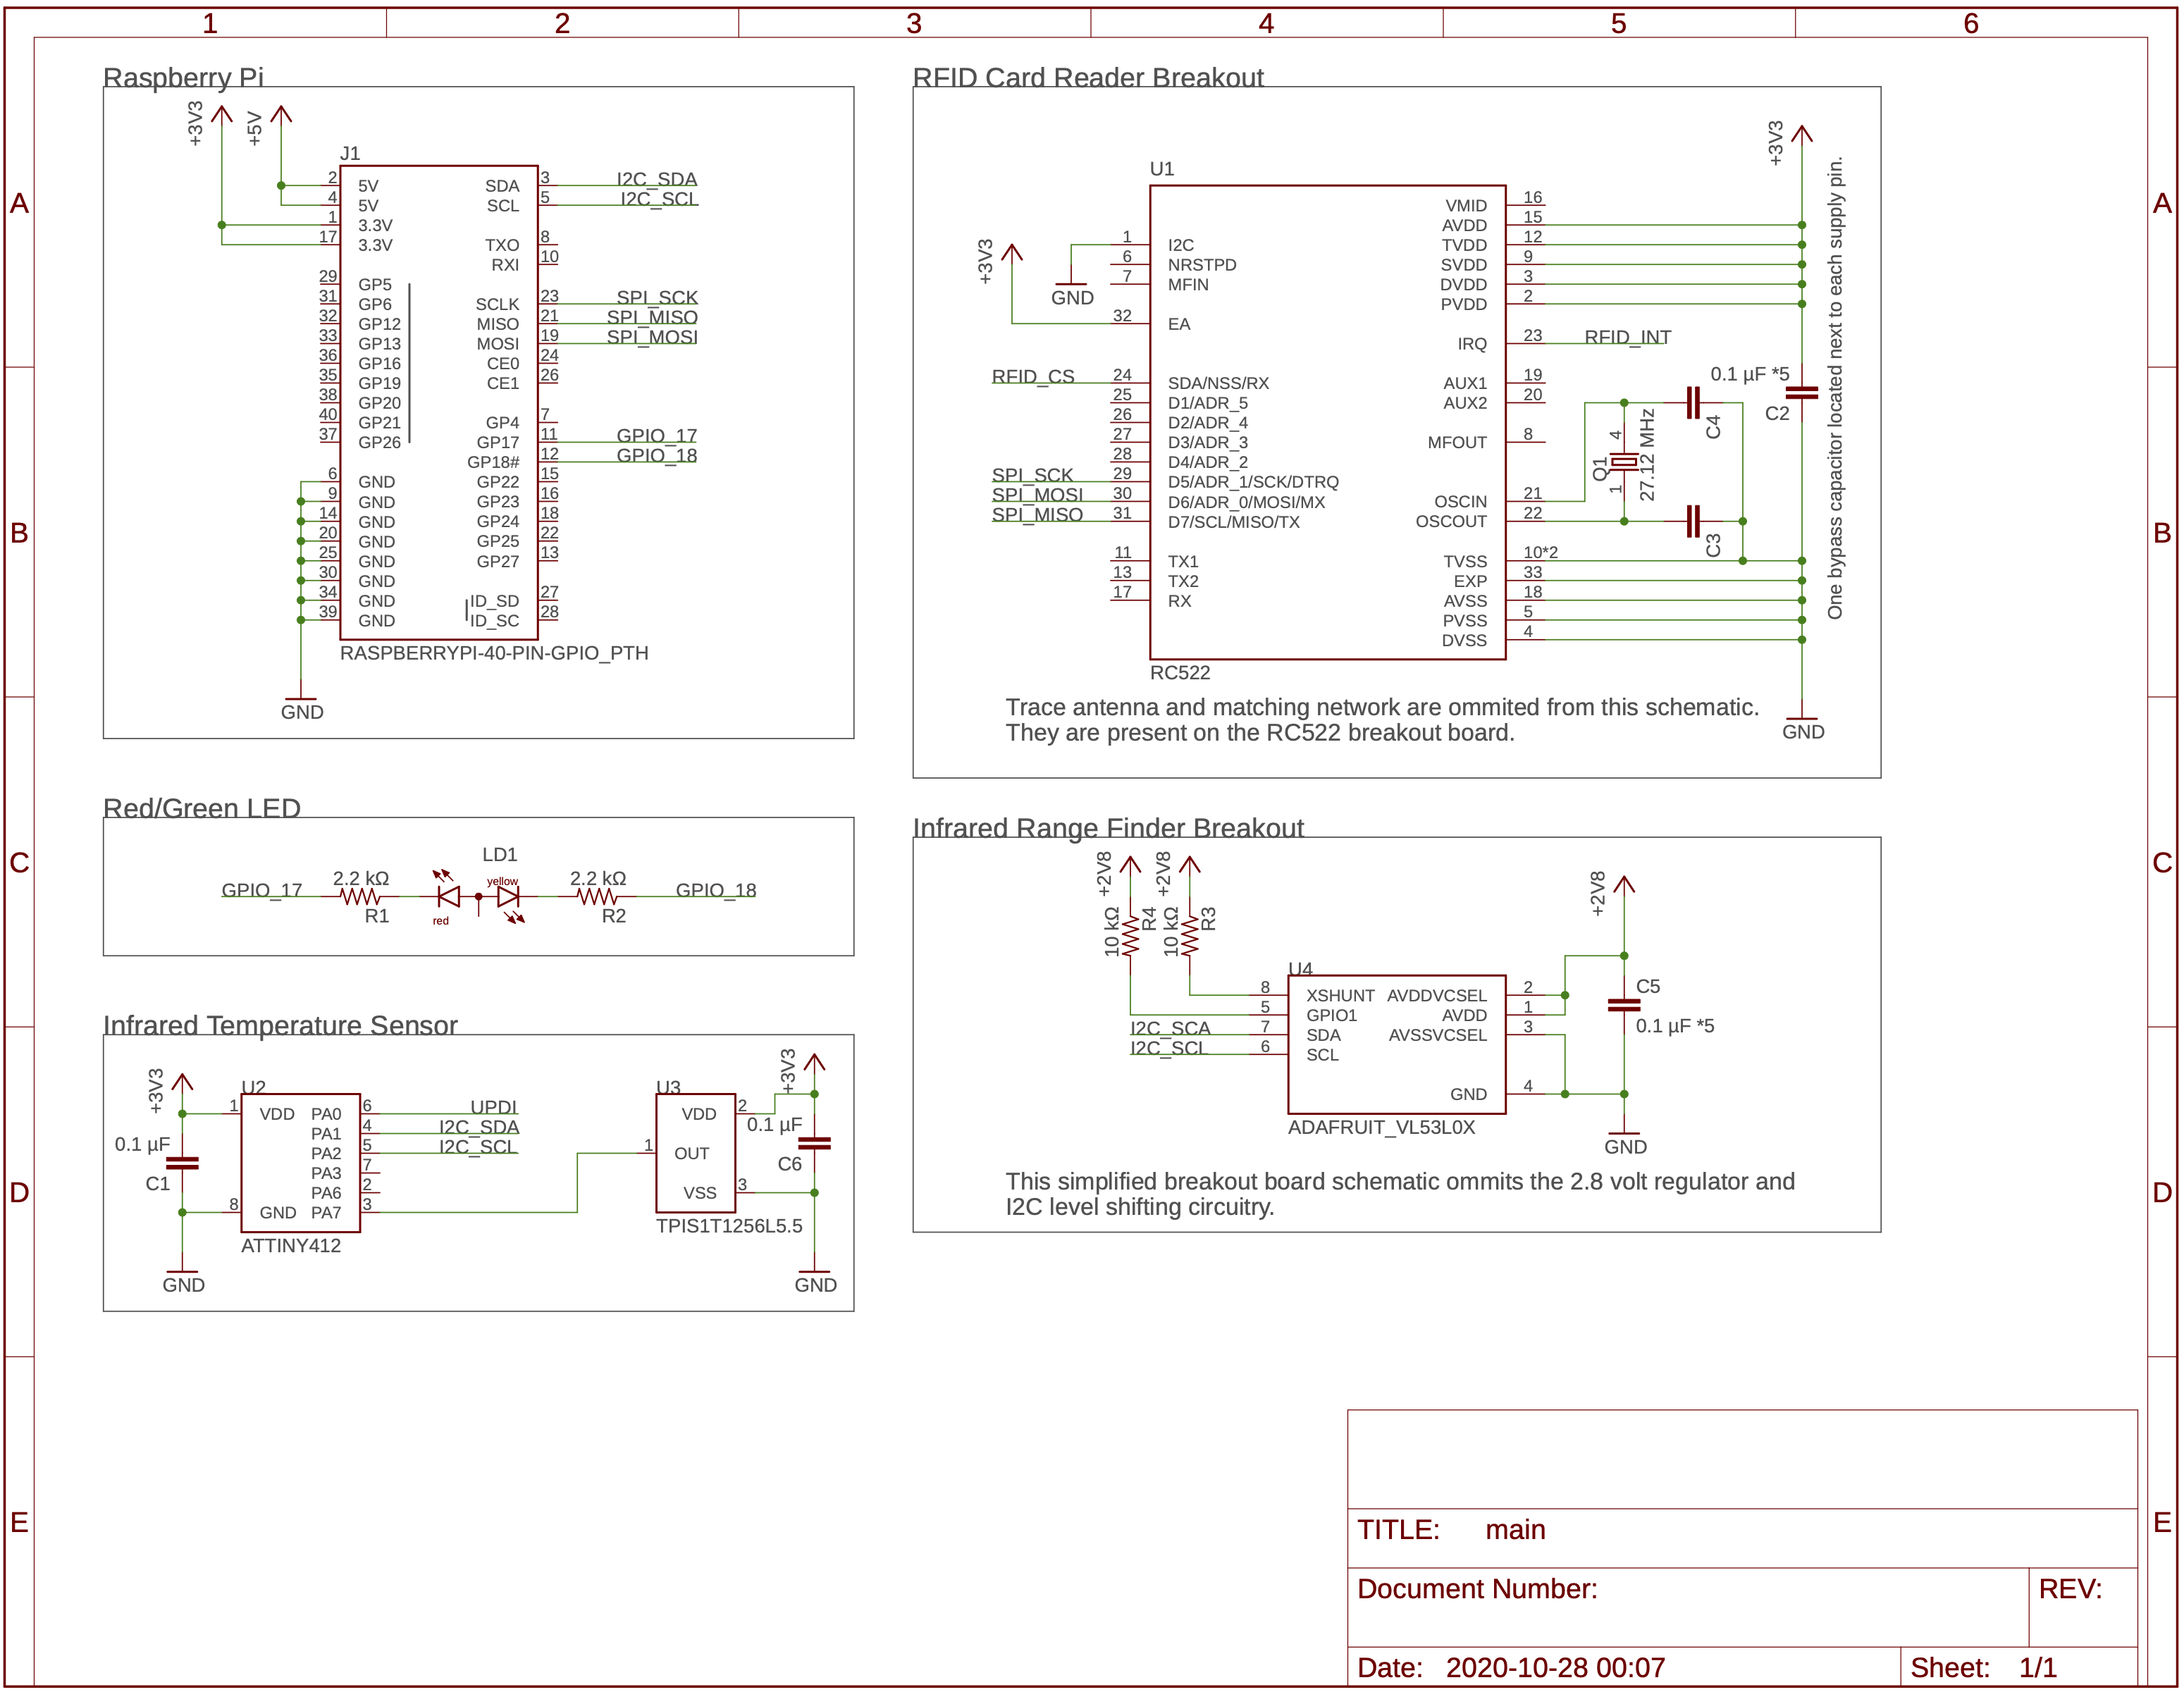
\includegraphics[width=\textwidth]{images/door-node-schematic.png}
\caption{Door Node Schematic}
\label{fig:door-node-schematic}
\end{figure}

\subsection{Infrared Temperature Sensor}

In order to detect fever we need to measure the temperature of the users of our
system. We have determined that a forehead temperature measurement using an
infrared temperature sensor is the best way to obtain sufficiently accurate
contactless temperature measurements.

We plan to use the MLX90614 thermopile from Melexis Technologies. This
temperature sensor was chosen after a comparison of available infrared
temperature sensors.

The MLX90614 offers medical grade accuracy within the temperature range expected
for human skin. It also provides accurate ambient temperature measurements. The
optics of the sensor provide a relatively narrow field of view which is
appropriate for measuring the fairly small target of a human forehead from a
reasonable range.

The MLX90614 can be powered from the Raspberry Pi's 3.3 volt rail and
features an I$^2$C serial interface, which is suitable for communication with a
Raspberry Pi.

Figure \ref{fig:ir-test-circuit} shows the test circuit for the infrared
temperature sensor.

\begin{figure}[!htb]
\centering
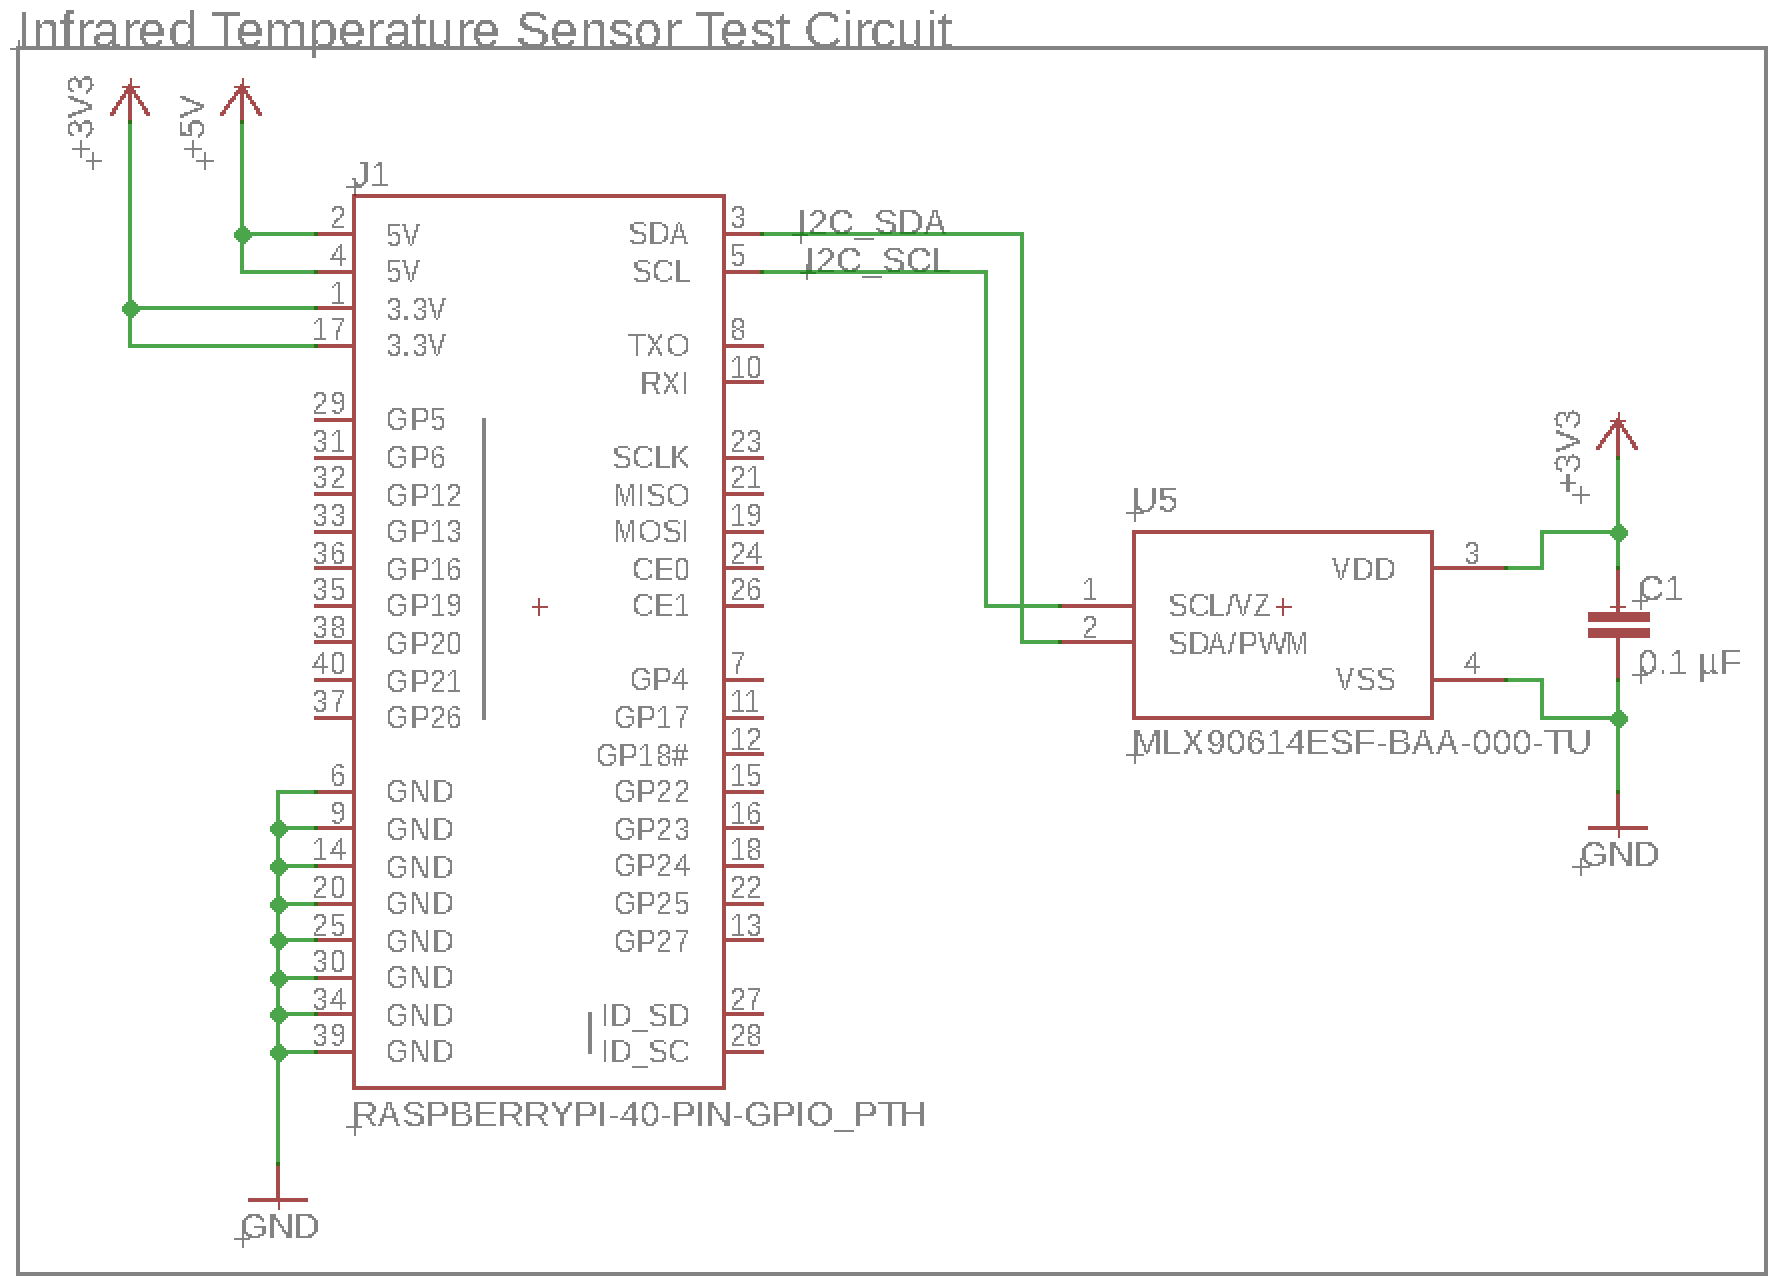
\includegraphics[width=0.75\textwidth]{images/ir-test-circuit.png}
\caption{Test Circuit for Infrared Temperature Sensor}
\label{fig:ir-test-circuit}
\end{figure}

\subsection{NFC Security Badge Reader}

The MFRC522 RFID reader is the chosen device for the NFC security badge reader. 
It has an operating distance of up to 50 mm which means that the users will not have to place
the card almost touching the reader. the fact that it includes a programmable timer
is very useful as it can help avoid creating issues where it scans a card multiple times 
when doing a single swipe. As the reader is not meant to be the end all of deciding 
whether or not an employee will unlock the door it is therefore useful that the device
supports power down by software mode. When in lockdown or an employee attempts
to enter the building at full capacity it will be powered-down preventing entrance.  
The usage of serial peripheral interface helps as the badge reader functions quickly 
being able to handle data speeds up to 10 Mbit/s. 
It is powered by the 3.3 V DC power source of the Raspberry Pi.


For the below test circuit the differences between the test circuit and the actual demo circuit
are as follows. The T GPIO extension board used is coloured differently
and indicates GPIO rather than "\#" before the numbers. 
Other then those two changes the below circuit is identical to that which will be used in demonstrations.

\begin{figure}[!htb]
\centering
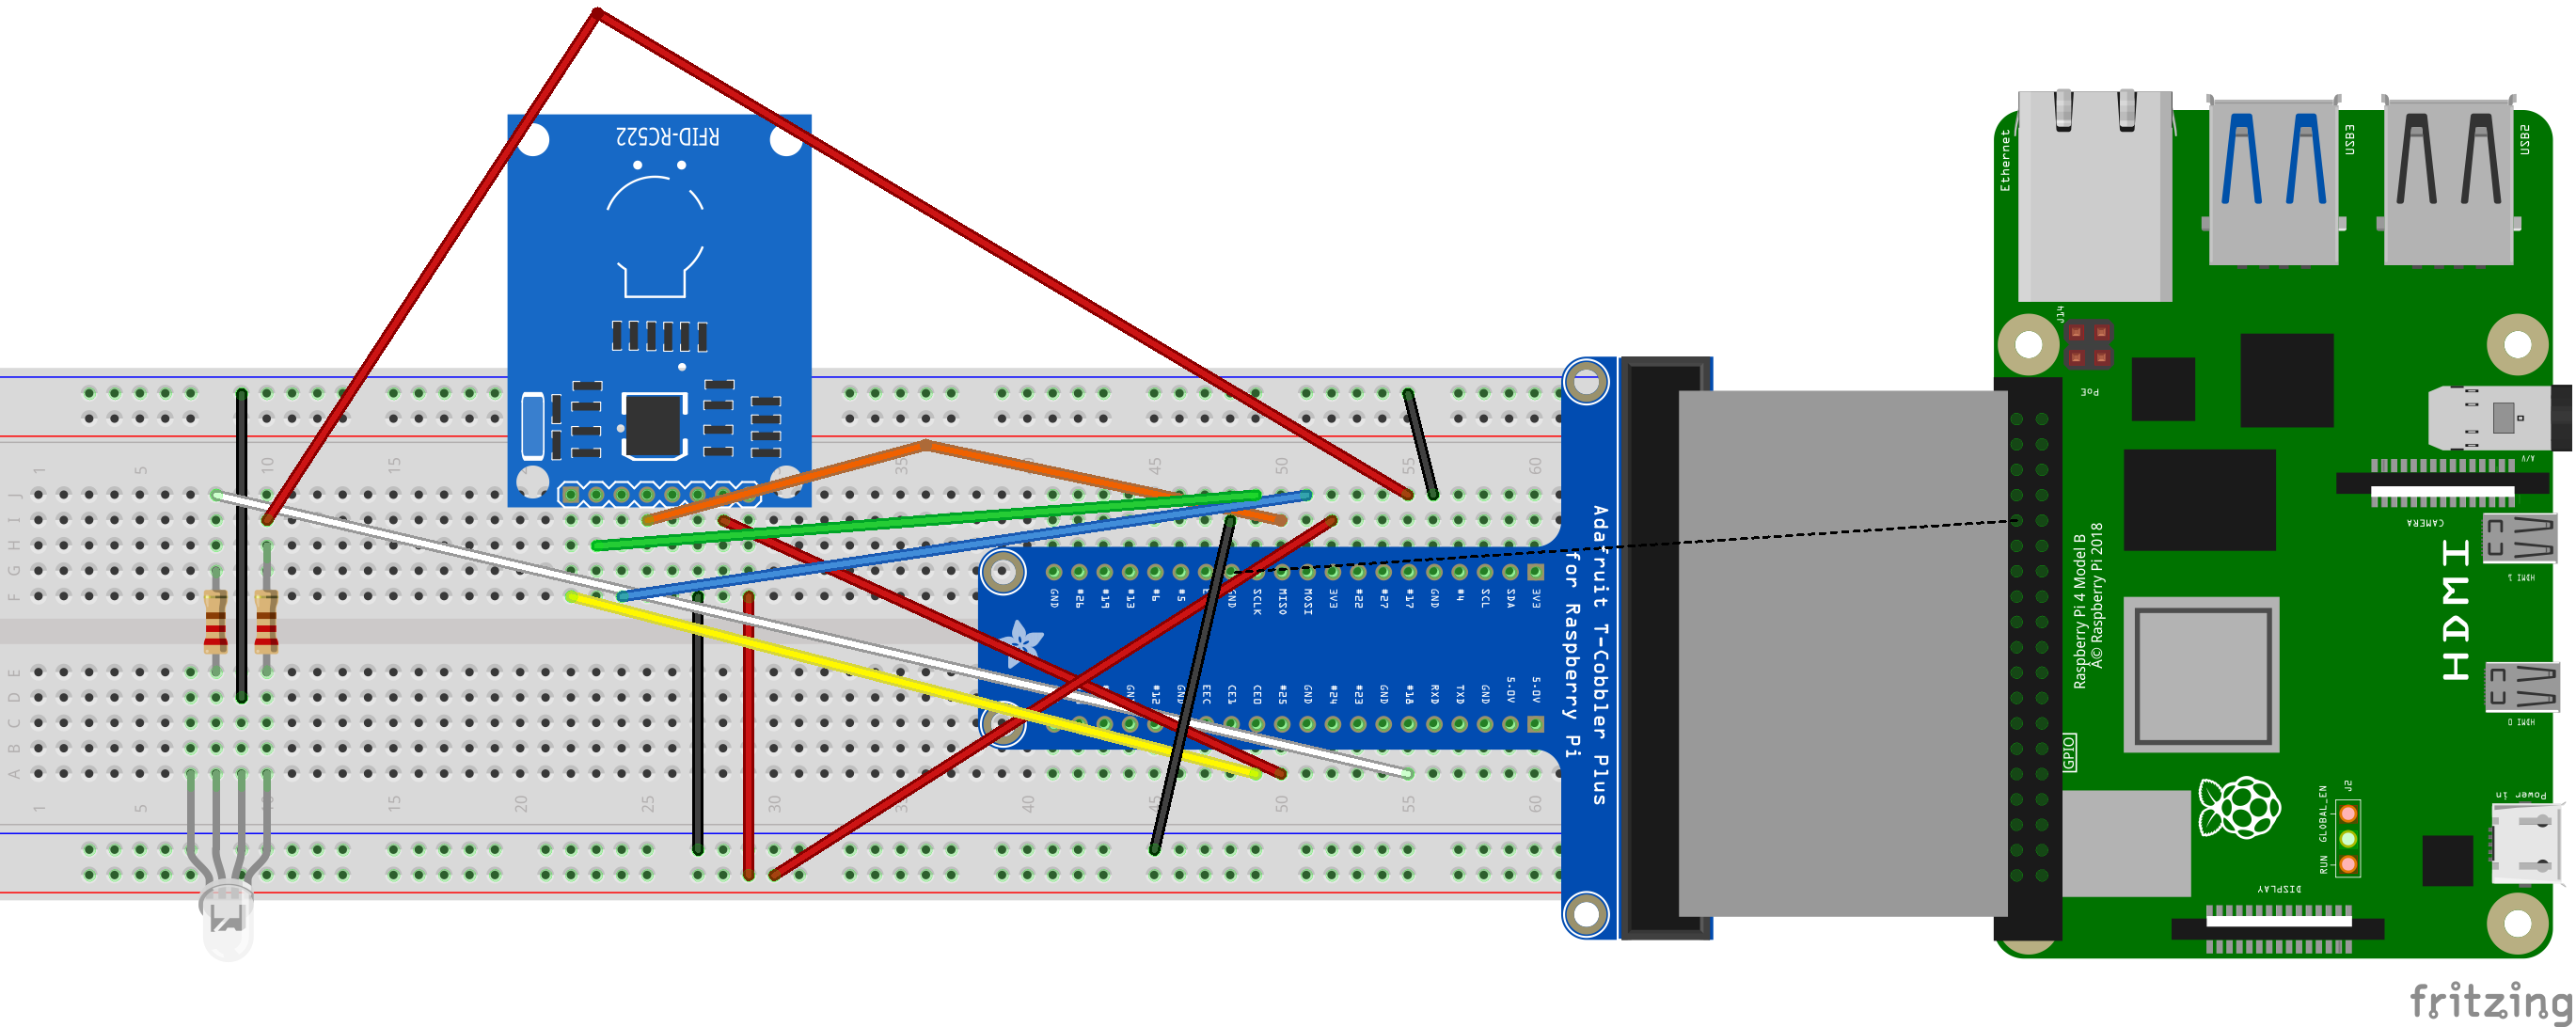
\includegraphics[width=\textwidth]{images/nfc-test-circuit.png}
\caption{Test Circuit for NFC Security Badge Reader}
\label{fig:nfc-test-circuit}
\end{figure}

\subsection{Electronic Door Lock}

The electronic door lock model will be powered by a servo motor. The chosen
servo motor is the Adafruit Micro Servo.  This servo has 180 degrees of motion
that can be traversed in 0.3 seconds.  The servo operates between 3V and 6V so
it can be powered through the Raspberry Pi's 5V line.

Figure \ref{fig:lock-test-circuit} shows the test circuit for the electronic
door lock.

\begin{figure}[!htb]
\centering
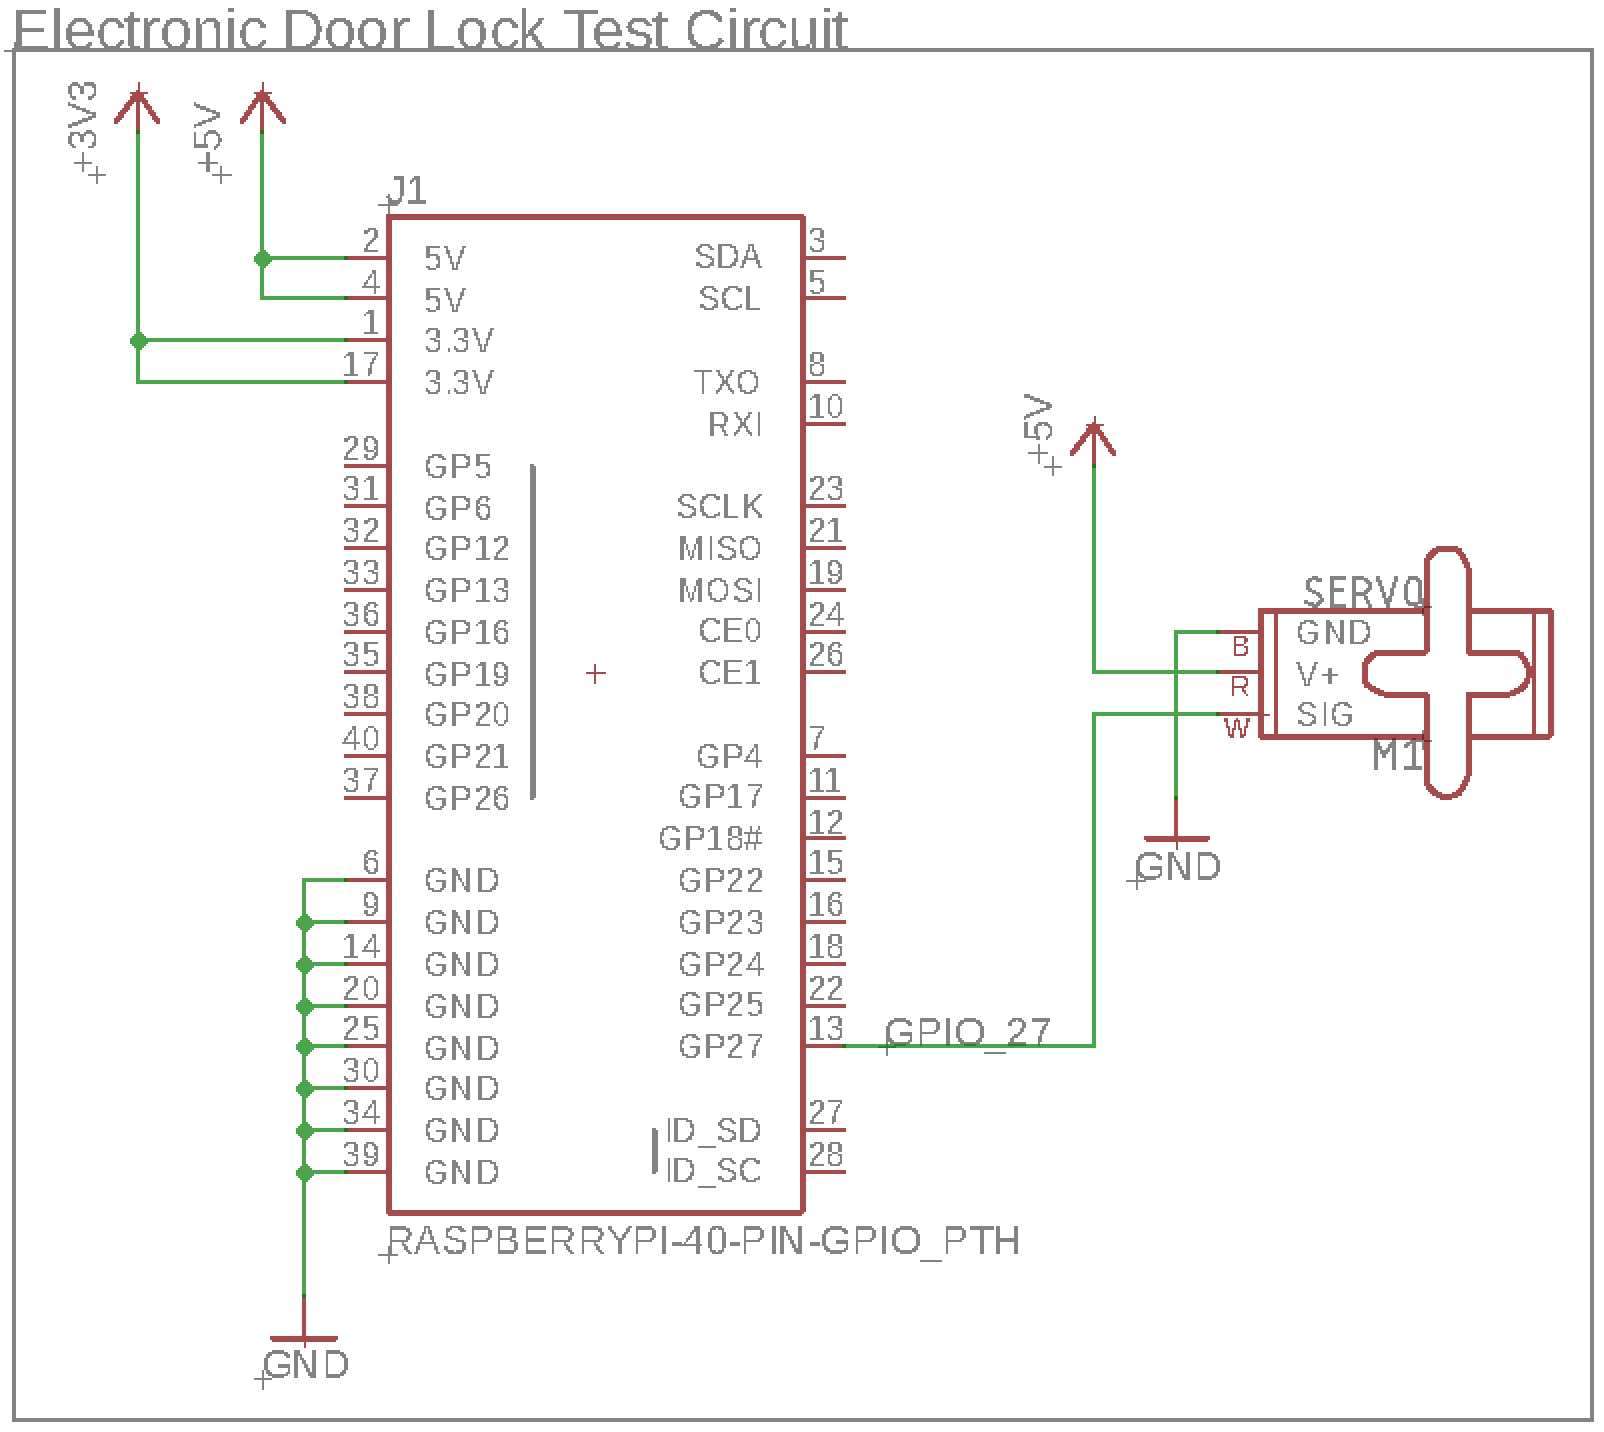
\includegraphics[width=0.75\textwidth]{images/lock-test-circuit.png}
\caption{Test Circuit for Electronic Door Lock}
\label{fig:lock-test-circuit}
\end{figure}

\subsection{Time of Flight Range Sensor}

\begin{figure}[!htb]
\centering
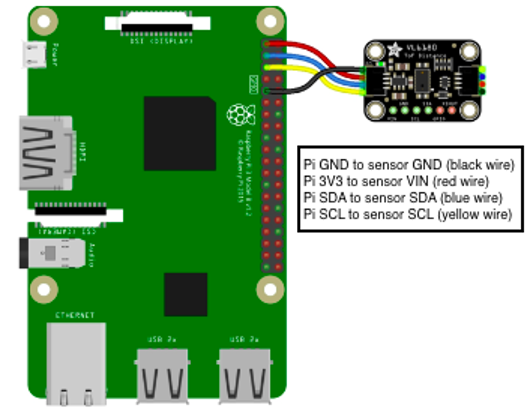
\includegraphics[width=0.6\textwidth]{images/tof-test-circuit.png}
\caption{Test Circuit for Time of Flight Sensor}
\label{fig:tof-test-circuit}
\end{figure}


\subsection{Control Server}

The control server hardware will consist of a Raspberry Pi connected to a
monitor, keyboard and mouse.


\clearpage

\section{Test Plan}
\label{sec:test-plan}
\subsection{End to End Demo}

\noindent
Software requirements:
\begin{itemize}
    \item Set up Thingspeak channel 
    \item Hard code sensor signal communication to Thingspeak 
    \item Have test stubs which emulate the functionality of the hardware
          components ready
\end{itemize}

\subsubsection*{Entry Access}

\paragraph{Scenario 1}
Building accepting entries, employee with valid NFC card, authorized status,
normal body temperature, ideal distance away from temperature sensor and
building accessible after entry.

\noindent
Features to be tested:
\begin{itemize}
    \item Communication between control server and Thingspeak
    \item Communication between door node and Thingspeak
\end{itemize}

\noindent
Test scenario steps:
\begin{enumerate}
    \item Control server checks for the number of people in the building and 
          sends an DOOR\_STATE\_UPDATE to Thingspeak channel
    \item Door node receives the DOOR\_STATE\_UPDATE from Thingspeak channel and 
          if available, displays green light to indicate door node accepting 
          entries on the LED display
    \item NFC reader identifies NFC id card being tapped and sends 
          ACCESS\_REQUEST with card id to Thingspeak channel
    \item Control server receives ACCESS\_REQUEST from Thingspeak channel and 
          validates NFC card id and identifies employee id by querying the 
          database for the NFC card id 
    \item Once acquiring the valid employee id, the control server queries the 
          database for recent employee status, access type and validity to 
          consider entry access
    \item If recent status is authorized, access type was exit and validity is
          less than 3, control server determines current access type to be 
          entry and sends INFROMATION\_REQUEST to determine if employee in 
          distance range to Thingspeak channel
    \item Door node receives INFROMATION\_REQUEST from the Thingspeak channel
          and activates the LED display and displays orange to indicate that the
          access entry process is in progress 
    \item Door node activates the rangefinder to identify users range from
          temperature sensor
    \item Door node records the range value and sends an INFORMATION\_RESPONSE
          to the Thingspeak channel
    \item Control server receives the INFORMATION\_RESPONSE and compares the
          received range value with the ideal range value
    \item If in ideal range, control server sends an INFORMATION\_REQUEST to
          measure the user’s body temperature
    \item Door node receives the INFORMATION\_REQUEST and activates the 
          temperature sensor to record the user’s body temperature 
    \item Door node then sends an INFROMATION\_RESPONSE with the recorded
          temperature measurement to the Thingspeak channel 
    \item Control server receives the INFORMATION\_RESPONSE from the Thingspeak
          channel
    \item Control server compares recorded temperature value to acceptable
          temperature range and determines the status of the entry request
    \item If in acceptable temperature range, control server updates the status
          of the employee to “authorized” and saves all the information for
          access entry in the database and sets the validity field to 0
    \item Control server increments the number of people in the building by 1
    \item Control server sends an ACCESS\_RESPONSE to the Thingspeak channel
    \item Control server re-evaluates the number of people in the building and
          sends a DOOR\_STATE\_UPDATE based on the accessibility status of the 
          building to the Thingspeak channel
    \item Door node receives the ACCESS\_REPONSE and DOOR\_STATE\_UPDATE from 
          the Thingspeak channel
    \item From ACCESS\_RESPONSE received by the door node, if access is
          authorized, door node activates LED display to display a flashing
          green light to indicate employee’s access has been authorized 
    \item Door node also unlocks the electronic lock for 30 seconds
    \item After 30 sec, Door node locks the electronic lock
    \item From the DOOR\_STATE\_UPDATE received by the door node, if the
          building is accessible, door node activates LED display to display a
          green light to indicate system is accepting entry
\end{enumerate}

\noindent
Expected test scenario result: proper communication between nodes and control
server occurred to authorize employee access to the workplace.


\paragraph{Scenario 2}
Building accepting entries, employee with valid NFC card, authorized status,
normal body temperature, ideal distance away from temperature sensor and
building not accessible after entry

\noindent
Features to be tested:
\begin{itemize}
    \item Communication between control server and Thingspeak
    \item Communication between door node and Thingspeak
\end{itemize}

\noindent
Test scenario steps:
\begin{enumerate}
    \item Control server checks for the number of people in the building and
          sends a DOOR\_STATE\_UPDATE to Thingspeak channel
    \item Door node receives the DOOR\_STATE\_UPDATE from Thingspeak channel and
          if available, displays green light to indicate door node accepting
          entries on the LED display
    \item NFC reader identifies NFC id card being tapped and sends
          ACCESS\_REQUEST with card id to Thingspeak channel
    \item Control server receives ACCESS\_REQUEST from Thingspeak channel and
          validates NFC card id and identifies employee id by querying the
          database for the NFC card id 
    \item Once acquiring the valid employee id, the control server queries the
          database for recent employee status, access type and validity to
          consider entry access
    \item If recent status is authorized, access type was exit and validity is
          less than 3, control server determines current access type to be entry
          and sends INFROMATION\_REQUEST to determine if employee in distance
          range to Thingspeak channel
    \item Door node receives INFROMATION\_REQUEST from the Thingspeak channel
          and activates the LED display and displays orange to indicate that the
          access entry process is in progress 
    \item Door node activates the rangefinder to identify users range from
          temperature sensor
    \item Door node records the range value and sends an INFORMATION\_RESPONSE
          to the Thingspeak channel
    \item Control server receives the INFORMATION\_RESPONSE and compares the
          received range value with the ideal range value
    \item If in ideal range, control server sends an INFORMATION\_REQUEST to
          measure the user’s body temperature
    \item Door node receives the INFORMATION\_REQUEST and activates the
          temperature sensor to record the user’s body temperature 
    \item Door node then sends an INFROMATION\_RESPONSE with the recorded
          temperature measurement to the Thingspeak channel 
    \item Control server receives the INFORMATION\_RESPONSE from the Thingspeak
          channel
    \item Control server compares recorded temperature value to acceptable
          temperature range and determines the status of the entry request
    \item If in acceptable temperature range, control server updates the status
          of the employee to “authorized” and saves all the information for
          access entry in the database and sets the validity field to 0
    \item Control server increments the number of people in the building by 1
    \item Control server sends an ACCESS\_RESPONSE to the Thingspeak channel
    \item Control server re-evaluates the number of people in the building and
          sends a DOOR\_STATE\_UPDATE based on the accessibility status of the
          building to the Thingspeak channel
    \item Door node receives the ACCESS\_REPONSE and DOOR\_STATE\_UPDATE from
          the Thingspeak channel
    \item From ACCESS\_RESPONSE received by the door node, if access is
          authorized, door node activates LED display to display a flashing
          green light to indicate employee’s access has been authorized 
    \item Door node also unlocks the electronic lock for 30 seconds
    \item After 30 sec, Door node locks the electronic lock
    \item From the DOOR\_STATE\_UPDATE received by the door node, if the
          building is not accessible, door node activates LED display to display
          a red light to indicate system is not accepting entry
\end{enumerate}

\noindent
Expected test scenario result: Proper communication between door node and
control server occurred to authorize employee access to the workplace and
restrict entry to additional employees after the process.

\paragraph{Scenario 3}
Building accepting entries, employee with invalid NFC card, authorized status,
normal body temperature, in ideal distance range away from temperature sensor at
entry node and building accessible after entry attempt.

\noindent
Features to be tested:
\begin{itemize}
    \item Communication between control server and Thingspeak
    \item Communication between door node and Thingspeak
\end{itemize}

\noindent
Test scenario steps:
\begin{enumerate}
    \item Control server checks for the number of people in the building and
          sends an DOOR\_STATE\_UPDATE to Thingspeak channel
    \item Door node receives the DOOR\_STATE\_UPDATE from Thingspeak channel and
         if available, displays green light to indicate door node accepting
         entries on the LED display
    \item NFC reader identifies NFC id card being tapped and sends
          ACCESS\_REQUEST with card id to Thingspeak channel
    \item Control server receives ACCESS\_REQUEST from Thingspeak channel and
          queries the database for the NFC card id to be associated to the
          employee id
    \item If no valid employee id acquired, the control server sends an
          ACCESS\_RESPONSE indicating invalid id card being scanned to the
          Thingspeak channel
    \item Control server re-evaluates the number of people in the building and
          sends a DOOR\_STATE\_UPDATE based on the accessibility status of the
          building to the Thingspeak channel
    \item Door node receives ACCESS\_RESPONSE and DOOR\_STATE\_UPDATE from the
          Thingspeak channel 
    \item From the ACCESS\_REPONSE received, door node locks the electronic
          lock and displays flashing red light to indicate that the access entry
          attempt is invalid
    \item From the DOOR]\_STATE\_UPDATE received by the door node, if the
          building is accessible, door node activates LED display to display a
          green light to indicate system is accepting entry
\end{enumerate}

\noindent
Expected test scenario result: proper communication between nodes and control
server occurred to unauthorize employee access to workplace.

\paragraph{Scenario 4}
Building accepting entries, employee with valid NFC card, authorized status,
normal body temperature, not in ideal distance range away from temperature
sensor and building accessible after entry attempt.

\noindent
Features to be tested:
\begin{itemize}
    \item Communication between control server and Thingspeak
    \item Communication between door node and Thingspeak
\end{itemize}

\noindent
Test scenario steps:
\begin{enumerate}
    \item Control server checks for the number of people in the building and
          sends an DOOR\_STATE\_UPDATE to Thingspeak channel
    \item Door node receives the DOOR\_STATE\_UPDATE from Thingspeak channel and
          if available, displays green light to indicate door node accepting
          entries on the LED display
    \item NFC reader identifies NFC id card being tapped and sends
          ACCESS\_REQUEST with card id to Thingspeak channel
    \item Control server receives ACCESS\_REQUEST from Thingspeak channel and
          validates NFC card id and identifies employee id by querying the
          database for the NFC card id 
    \item Once acquiring the valid employee id, the control server queries the
          database for recent employee status, access type and validity to
          consider entry access
    \item If recent status is authorized, access type was exit and validity is
          less than 3, control server determines current access type to be entry
          and sends INFROMATION\_REQUEST to determine if employee in distance
          range to Thingspeak channel and increments validity by 1
    \item Door node receives INFROMATION\_REQUEST from the Thingspeak channel
          and activates the LED display and displays orange to indicate that
          the access entry process is in progress 
    \item Door node activates the rangefinder to identify users range from
          temperature sensor
    \item Door node records the range value and sends an INFORMATION\_RESPONSE
          to the Thingspeak channel
    \item Control server receives the INFORMATION\_RESPONSE and compares the
          received range value with the ideal range value
    \item Since not in ideal range, control server checks the validity field to
          see if its less than 3, if yes then it sends an INFORMATION\_REQUEST
          to check again if employee in range and increments the validity by 1 
    \item Door node receives the INFORMATION\_REQUEST from the Thingspeak
          channel and activates the rangefinder again to identify if employee in
          range of temperature sensor
    \item Door node sends an INFORMATION\_RESPONSE with the recorded range value
    \item Control server receives the INFORMATION\_RESPONSE from the Thingspeak
          channel and compares the received range value with the ideal range
          value
    \item Since not in ideal range, control server checks the validity field to
          see if its less than 3, if yes then it sends an INFORMATION\_REQUEST
          to check again if employee in range and increments the validity by 1 
    \item Door node receives the INFORMATION\_REQUEST and activates the
          rangefinder again to identify if employee in range of temperature
          sensor
    \item Door node sends an INFORMATION\_RESPONSE with recorded range value to
          the Thingspeak channel
    \item Control server receives the INFORMATION\_RESPONSE from the Thingspeak
          channel and compares the received range value with the ideal range
          value 
    \item Since not in ideal range, control server checks the validity field to
          see if its less than 3, if not less than 3 then control serveri
          determines the access entry is invalid and determines the
          ACCESS\_RESPONSE to be sent
    \item control server updates the validity field for the access entry to 3
          and saves all the information for access entry in the database
    \item Control server re-evaluates the number of people in the building and
          sends a DOOR\_STATE\_UPDATE based on the accessibility status of the
          building to the Thingspeak channel
    \item Door node receives the ACCESS\_REPONSE and DOOR\_STATE\_UPDATE from
          the Thingspeak channel
    \item From ACCESS\_RESPONSE received by the door node, since access is
          invalid, door node locks the electronic lock and displays a red light
          to indicate access denied 
    \item From the DOOR\_STATE\_UPDATE received by the door node, if the
          building is accessible, door node activates LED display to display a
          green light to indicate system is accepting entry
\end{enumerate}

\noindent
Expected test scenario result: Proper communication between door node and
control server occurred to let the employee know to stand in an ideal distance
range away from the temperature sensor.

\paragraph{Scenario 5}
Building accepting entries, employee with valid NFC card, authorized status, in
ideal distance range away from temperature sensor, body temperature indicating
fever and building accessible after entry attempt.

\noindent
Features to be tested:
\begin{itemize}
    \item Communication between control server and Thingspeak
    \item Communication between door node and Thingspeak
\end{itemize}

\noindent
Test scenario steps:
\begin{enumerate}
    \item Control server checks for the number of people in the building and
          sends an DOOR\_STATE\_UPDATE to Thingspeak channel
    \item Door node receives the DOOR\_STATE\_UPDATE from Thingspeak channel and
          if available, displays green light to indicate door node accepting
          entries on the LED display
    \item NFC reader identifies NFC id card being tapped and sends
          ACCESS\_REQUEST with card id to Thingspeak channel
    \item Control server receives ACCESS\_REQUEST from Thingspeak channel and
          validates NFC card id and identifies employee id by querying the
          database for the NFC card id 
    \item Once acquiring the valid employee id, the control server queries the
          database for recent employee status, access type and validity to
          consider entry access
    \item If recent status is authorized, access type was exit and validity is
          less than 3, control server determines current access type to be entry
          and sends INFROMATION\_REQUEST to determine if employee in distance
          range to Thingspeak channel
    \item Door node receives INFROMATION\_REQUEST from the Thingspeak channel
          and activates the LED display and displays orange to indicate that the
          access entry process is in progress 
    \item Door node activates the rangefinder to identify users range from
          temperature sensor
    \item Door node records the range value and sends an INFORMATION\_RESPONSE
          to the Thingspeak channel
    \item Control server receives the INFORMATION\_RESPONSE and compares the
          received range value with the ideal range value
    \item If in ideal range, control server sends an INFORMATION\_REQUEST to
          measure the user’s body temperature
    \item Door node receives the INFORMATION\_REQUEST and activates the
          temperature sensor to record the user’s body temperature 
    \item Door node then sends an INFROMATION\_RESPONSE with the recorded
          temperature measurement to the Thingspeak channel 
    \item Control server receives the INFORMATION\_RESPONSE from the Thingspeak
          channel
    \item Control server compares recorded temperature value to acceptable
          temperature range and determines the status of the entry request
    \item If not in acceptable temperature range, control server checks the
          validity field to see if its less than 3, if yes then it sends an
          INFORMATION\_REQUEST to measure the user body temperature again and
          increments the validity by 1 
    \item Door node receives the INFORMATION\_REQUEST from the Thingspeak
          channel and activates the temperature sensor again to record user body
          temperature
    \item Door node sends an INFORMATION\_RESPONSE with the recorded body
          temperature value
    \item Control server receives the INFORMATION\_RESPONSE from the Thingspeak
          channel and compares the received temperature value with the ideal
          temperature value
    \item Since not in ideal range, control server checks the validity field to
          see if its less than 3, if yes then it sends an INFORMATION\_REQUEST
          to record user body temperature again and increments the validity by 1 
    \item Door node receives the INFORMATION\_REQUEST and activates the
          temperature sensor again to record body temperature of user
    \item Door node sends an INFORMATION\_RESPONSE with recorded temperature
          value to the Thingspeak channel
    \item Control server receives the INFORMATION\_RESPONSE from the Thingspeak
          channel and compares the received temperature value with the ideal
          temperature value 
    \item Since not in ideal range, control server checks the validity field to
          see if its less than 3, if not less than 3 then control server
          determines the access entry is invalid and determines the
          ACCESS\_RESPONSE to be sent
    \item control server updates the validity field for the access entry to 3,
          updates the status to unauthorized and saves all the information for
          access entry in the database
    \item Control server re-evaluates the number of people in the building and
          sends a DOOR\_STATE\_UPDATE based on the accessibility status of the
          building to the Thingspeak channel
    \item Door node receives the ACCESS\_REPONSE and DOOR\_STATE\_UPDATE from
          the Thingspeak channel
    \item From ACCESS\_RESPONSE received by the door node, since access is
          unauthorized, door node locks the electronic lock and displays a
          flashing red light to indicate access denied 
    \item From the DOOR\_STATE\_UPDATE received by the door node, if the
          building is accessible, door node activates LED display to display a
          green light to indicate system is accepting entry
\end{enumerate}

\noindent
Expected test scenario result: Proper communication between nodes and control
server occurred to unauthorize employee and restrict access to workplace.

\paragraph{Scenario 6}
Building not accepting entries, employee with invalid NFC card, authorized
status, in ideal distance range, normal body temperature and building accessible
after entry attempt.

\noindent
Features to be tested:
\begin{itemize}
    \item Communication between control server and Thingspeak
    \item Communication between door node and Thingspeak
\end{itemize}

\noindent
Test scenario steps:
\begin{enumerate}
    \item Control server checks for the number of people in the building and
          sends a DOOR\_STATE\_UPDATE to Thingspeak channel
    \item Door node receives the DOOR\_STATE\_UPDATE from Thingspeak channel and
          since entry not available, displays red light to indicate door node
          not accepting entries on the LED display
    \item NFC reader identifies NFC id card being tapped and sends
          ACCESS\_REQUEST with card id to Thingspeak channel
    \item Control server receives ACCESS\_REQUEST from Thingspeak channel and
          validates NFC card id and identifies employee id by querying the
          database for the NFC card id 
    \item Once acquiring the valid employee id, the control server queries the
          database for recent employee status, access type and validity to
          consider entry access
    \item If recent status is authorized, access type was exit and validity is
          less than 3, control server determines current access type to be entry
          and sends INFROMATION\_REQUEST to determine if employee in distance
          range to Thingspeak channel
    \item Control server receives ACCESS\_REQUEST from Thingspeak channel and
          since building not the control server sends an ACCESS\_RESPONSE
          indicating entry not available
    \item Control server re-evaluates the number of people in the building and
          sends a DOOR\_STATE\_UPDATE based on the accessibility status of the
          building to the Thingspeak channel
    \item Door node receives ACCESS\_RESPONSE and DOOR\_STATE\_UPDATE from the
          Thingspeak channel 
    \item From the ACCESS\_REPONSE received, door node locks the electronic lock
          and displays red light to indicate building not accepting entries 
    \item From the DOOR\_STATE\_UPDATE received by the door node, since building
          still not accessible, door node activates LED display to display a red
          light to indicate system is not accepting entry
\end{enumerate}

\noindent
Expected test scenario result: Proper communication between door node and
control server occurred to let the employee know entry not available.

\paragraph{Scenario 7}
Building accepting entries, employee with invalid NFC card, unauthorized status 
(over 14 days ago), in ideal distance range away from temperature sensor, normal
body temperature and building accessible after entry attempt.

\noindent
Features to be tested:
\begin{itemize}
    \item Communication between control server and Thingspeak
    \item Communication between door node and Thingspeak
\end{itemize}

\noindent
Test scenario steps:
\begin{enumerate}
    \item Control server checks for the number of people in the building and
          sends a DOOR\_STATE\_UPDATE to Thingspeak channel
    \item Door node receives the DOOR\_STATE\_UPDATE from Thingspeak channel and
          if available, displays green light to indicate door node accepting
          entries on the LED display
    \item NFC reader identifies NFC id card being tapped and sends
          ACCESS\_REQUEST with card id to Thingspeak channel
    \item Control server receives ACCESS\_REQUEST from Thingspeak channel and
          validates NFC card id and identifies employee id by querying the
          database for the NFC card id 
    \item Once acquiring the valid employee id, the control server queries the
          database for recent employee status, access type and validity to
          consider entry access
    \item If recent status is unauthorized, access type was entry and validity
          is 3, control server determines current access type to be entry and
          queries the database for date of most recent entry attempt
    \item If most recent entry attempt date over 14 days ago, control server
          sends INFROMATION\_REQUEST to determine if employee in distance range
          to Thingspeak channel
    \item Door node receives INFROMATION\_REQUEST from the Thingspeak channel
          and activates the LED display and displays orange to indicate that the
          access entry process is in progress 
    \item Door node activates the rangefinder to identify users range from
          temperature sensor
    \item Door node records the range value and sends an INFORMATION\_RESPONSE 
          to the Thingspeak channel
    \item Control server receives the INFORMATION\_RESPONSE and compares the
          received range value with the ideal range value
    \item If in ideal range, control server sends an INFORMATION\_REQUEST to
          measure the user’s body temperature
    \item Door node receives the INFORMATION\_REQUEST and activates the
          temperature sensor to record the user’s body temperature 
    \item Door node then sends an INFROMATION\_RESPONSE with the recorded
          temperature measurement to the Thingspeak channel 
    \item Control server receives the INFORMATION\_RESPONSE from the Thingspeak
          channel
    \item Control server compares recorded temperature value to acceptable
          temperature range and determines the status of the entry request
    \item If in acceptable temperature range, control server updates the status
          of the employee to “authorized” and saves all the information for
          access entry in the database and sets the validity field to 0
    \item Control server increments the number of people in the building by 1
    \item Control server sends an ACCESS\_RESPONSE to the Thingspeak channel
    \item Control server re-evaluates the number of people in the building and
          sends a DOOR\_STATE\_UPDATE based on the accessibility status of the
          building to the Thingspeak channel
    \item Door node receives the ACCESS\_REPONSE and DOOR\_STATE\_UPDATE from
          the Thingspeak channel
    \item From ACCESS\_RESPONSE received by the door node, if access is
          authorized, door node activates LED display to display a flashing
          green light to indicate employee’s access has been authorized 
    \item Door node also unlocks the electronic lock for 30 seconds
    \item After 30 sec, Door node locks the electronic lock
    \item From the DOOR\_STATE\_UPDATE received by the door node, if the
          building is accessible, door node activates LED display to display a
          green light to indicate system is accepting entry
\end{enumerate}

\noindent
Expected test scenario result: Proper communication between door node and
control server occurred to authorize employee access to the workplace.

\paragraph{Scenario 8}
Building accepting entries, employee with invalid NFC card, unauthorized status
(not over 14 days ago), in ideal distance range away from temperature sensor,
normal body temperature and building accessible after entry attempt.

\noindent
Features to be tested:
\begin{itemize}
    \item Communication between control server and Thingspeak
    \item Communication between door node and Thingspeak
\end{itemize}

\noindent
Test scenario steps:
\begin{enumerate}
    \item Control server checks for the number of people in the building and
          sends an DOOR\_STATE\_UPDATE to Thingspeak channel
    \item Door node receives the DOOR\_STATE\_UPDATE from Thingspeak channel and
          if available, displays green light to indicate door node accepting
          entries on the LED display
    \item NFC reader identifies NFC id card being tapped and sends
          ACCESS\_REQUEST with card id to Thingspeak channel
    \item Control server receives ACCESS\_REQUEST from Thingspeak channel and
          validates NFC card id and identifies employee id by querying the
          database for the NFC card id 
    \item Once acquiring the valid employee id, the control server queries the
          database for recent employee status, access type and validity to
          consider entry access
    \item If recent status is unauthorized, access type was entry and validity
          is 3, control server determines current access type to be entry and
          queries the database for date of most recent entry attempt
    \item If most recent entry attempt date not over 14 days ago, control server
          sends ACCESS\_RESPONSE indicated access unauthorized to the Thingspeak
          channel and no information for the entry attempt is saved in the
          database
    \item Control server re-evaluates the number of people in the building and
          sends a DOOR\_STATE\_UPDATE based on the accessibility status of the
          building to the Thingspeak channel
    \item Door node receives the ACCESS\_REPONSE and DOOR\_STATE\_UPDATE from
          the Thingspeak channel
    \item From ACCESS\_RESPONSE received by the door node, since access is
          unauthorized, door node locks the electronic lock and displays a
          flashing red light to indicate access denied 
    \item From the DOOR\_STATE\_UPDATE received by the door node, if the
          building is accessible, door node activates LED display to display a
          green light to indicate system is accepting entry
\end{enumerate}

\noindent
Expected test scenario result: Proper communication between door node and
control server occurred to let the employee know invalid access entry attempt.

\paragraph{Scenario 9}
Employee with valid NFC card and at exit node.

\noindent
Features to be tested:
\begin{itemize}
    \item Communication between control server and Thingspeak
    \item Communication between door node and Thingspeak
\end{itemize}

\noindent
Test scenario steps:
\begin{enumerate}
    \item NFC reader identifies NFC id card being tapped and sends
          ACCESS\_REQUEST with card id to Thingspeak channel
    \item Control server receives ACCESS\_REQUEST from Thingspeak channel and
          validates NFC card id and identifies employee id by querying the
          database for the NFC card id 
    \item Once acquiring the valid employee id, the control server queries the
          database for recent employee status, access type and validity toi
          consider entry access
    \item If recent status is authorized, access type was entry and validity is
          3 or less than 3, control server determines current access type to be
          exit 
    \item If most recent access type is entry attempt control server sends
          ACCESS\_RESPONSE indicated exit access to the Thingspeak channel, logs
          information for the exit attempt in the database and subtracts1 from
          the number of people in the building  
    \item Control server re-evaluates the number of people in the building and
          sends a DOOR\_STATE\_UPDATE based on the accessibility status of the
          building to the Thingspeak channel
    \item Door node receives the ACCESS\_REPONSE and DOOR\_STATE\_UPDATE from
          the Thingspeak channel
    \item From ACCESS\_RESPONSE received by the door node, since access type is
          exit, door node unlocks the electronic lock at exit node 
    \item From the DOOR\_STATE\_UPDATE received by the door node, if the
          building is accessible, door node activates LED display to display a
          green light to indicate system is accepting entry
\end{enumerate}

\noindent
Expected test scenario result:Employee successfully exits the building an
accessibility of building updated.   

\subsection{Testing Demo}

\subsubsection{Hardware Tests}

\paragraph{Infrared Temperature Sensor}

Table \ref{table:ir-tests} shows the test cases that will be used to test the
infrared temperature sensor.

\begin{longtable}[htb]{>{\centering\arraybackslash}m{0.75cm}|>{\centering\arraybackslash}m{4cm}|>{\centering\arraybackslash}m{4.5cm}|>{\centering\arraybackslash}m{4cm}}
\toprule
Test & Description & Setup & Expected Result \\
\midrule
1 & Measure a temperature within the normal range & Aim temperature sensor at
someone's forehead and take a measurement & Measured temperature value is within
the expected range \\
\hline
2 & Measure a temperature that could indicate a fever & Aim the temperature
sensor at a pot of water that has been heated to 39 ℃ and take a measurement &
Measured temperature value should be with 0.5 ℃ of 39 ℃. \\
\hline
3 & Measure a temperature below the expected range & Aim the temperature sensor
at any room temperature surface and take a measurement & The measurement should
be approximately room temperature. \\
\bottomrule
\caption{Infrared Temperature Sensor Tests}
\label{table:ir-tests}
\end{longtable}

\paragraph{NFC Security Badge Reader}

Table \ref{table:nfc-tests} shows the test cases that will be used to test the
NFC security badge reader.

\begin{longtable}[htb]{>{\centering\arraybackslash}m{0.75cm}|>{\centering\arraybackslash}m{4cm}|>{\centering\arraybackslash}m{4.5cm}|>{\centering\arraybackslash}m{4cm}}
\toprule
Test & Description & Setup & Expected Result \\
\midrule
1 & Green RGB LED functions & Have breadboard set up & Green is shown on LED \\
\hline
2 & Red RGB LED functions & Have breadboard set up & Red is shown on LED \\
\hline
3 & Green RGB LED can change to red & Have breadboard set up & Initially green
is shown on LED which then changes to red \\
\hline
4 & Red RGB LED can change to green & Have breadboard set up & Initially red is
shown on LED which then changes to green \\
\hline
5 & MFRC 522 RFID Module activates & Have breadboard set up. Have a passive tag
ready to wave in front & Pi prints out data on RFID tag \\
\hline
6 & MFRC 522 RFID Module can note separate ID & Have breadboard set up. Have two
passive tags ready to wave in front & Pi prints out different data for each RFID
tag swiped in front. \\
\hline
7 & MFRC 5222 RFID Module will not read when RGB LED is red & Have breadboard
set up. Have a passive tag ready to wave in front & RGB LED is red and no data
is printed out by the Pi. \\
\bottomrule
\caption{NFC Security Badge Reader Sensor Tests}
\label{table:nfc-tests}
\end{longtable}

\paragraph{Electronic Door Lock}

Table \ref{table:servo-tests} shows the test cases that will be used to test the
electronic door lock.

\begin{longtable}[htb]{>{\centering\arraybackslash}m{0.75cm}|>{\centering\arraybackslash}m{4cm}|>{\centering\arraybackslash}m{4.5cm}|>{\centering\arraybackslash}m{4cm}}
\toprule
Test & Description & Setup & Expected Result \\
\midrule
1 & Test servo Oscillation & Have breadboard set up & Servo alternates between
0 degrees and 180 degrees every second \\
\bottomrule
\caption{Electronic Door Lock Tests}
\label{table:servo-tests}
\end{longtable}

A test program will be written that will initially place the servo at an angle
of 0 degrees.  Then a loop will run that will move the servo arm to 180 degrees,
wait a second, move back to 0 degrees, and wait another second.  The operation
of the servo can be easily verified visually.

\paragraph{Time of Flight Range Sensor}

Table \ref{table:tof-tests} shows the test cases that will be used to test the
time of flight range sensor.

\begin{longtable}[htb]{>{\centering\arraybackslash}m{0.75cm}|>{\centering\arraybackslash}m{4cm}|>{\centering\arraybackslash}m{4.5cm}|>{\centering\arraybackslash}m{4cm}}
\toprule
Test & Description & Setup & Expected Result \\
\midrule
1 & Orange\_LED function activated & Have LED display set up with the Raspberry
Pi connected to monitor & RGB LED displays Orange \\
\hline
2 & Red\_LED function activated & Have LED display set up with the Raspberry Pi
connected to monitor & RGB LED displays Red \\
\hline
3 & Switch between orange and red LEDs & Have LED display set up with the
Raspberry Pi connected to monitor & RGB LED initially displays orange and then
switches to display red \\
\hline
4 & Switch between red and orange LEDs & Have LED display set up with the
Raspberry Pi connected to monitor & RGB LED initially displays red and then
switches to display orange \\
\hline
5 & VL6180X module activated & Have sensor connected to the Raspberry Pi and
connect Raspberry Pi to a display & Display prints out initial reading \\
\hline
6 & VL6180X module activated and Range\_Find class used to display multiple
range recordings & Have sensor connected to the Raspberry Pi and connect
Raspberry Pi to a display. Keep moving hand over the sensor to be able to
measure range. & Display prints out different readings recorded from moving
hand over the sensor \\
\bottomrule
\caption{Time of Flight Sensor Tests}
\label{table:tof-tests}
\end{longtable}

\subsubsection{Software Tests}

\subsubsection{Database Tests}

The following features are to be tested in order to test the integrity of the
database:

\begin{itemize}
    \item Control server populating right tables 
    \item Proper formatted data uploaded to appropriate fields
    \item Records of the temperature readings of all employees are accessible
          for at least 14 days
\end{itemize}

\paragraph{Scenario 1}
Populating sample test data access\_entry table.

\noindent
Features to be tested:
\begin{itemize}
    \item Control server populating right tables
\end{itemize}

\noindent
Initial setup: set up Raspberry pi connected to monitor keyboard and mouse.
Open command prompt on Raspberry Pi.

\noindent
Test scenario steps:
\begin{enumerate}
    \item Invoke SQLite by typing this command in the command prompt
\begin{lstlisting}
sqlite3
\end{lstlisting}
    \item Open the database by typing this command 
\begin{listing}[H]
\begin{minted}[]{text}
.open project_database.db
\end{minted}
\end{listing}
    \item Populate data to employee access\_entry table
\begin{listing}[H]
\begin{minted}[]{sql}
INSERT INTO access_entry
    VALUES(19234,time('now'),date('now'), "S_entry",
           "Yes", 38.0, "Authorized");
INSERT INTO access_entry
    VALUES(19437,time('now','-12 minutes'),date('now'),
          "E_entry", "Yes", 38.3, "Authorized");
INSERT INTO access_entry
    VALUES(19632,time('now','-1 hour'),date('now'),
           "N_entry", "Yes", 39.2, "Unauthorized");
INSERT INTO access_entry
    VALUES(19957,time('now','-5 minutes'),date('now'),
           "W_entry", "Yes", 38.5, "Authorized");
\end{minted}
\end{listing}
    \item Query data using \lstinline{Select*} command
\begin{listing}[H]
\begin{minted}[]{sql}
SELECT * FROM access_entry;
\end{minted}
\end{listing}
\end{enumerate}

\noindent
Expected test scenario result: table populated with test sample data and query
outputs.

\begin{lstlisting}
19234 | 09:30:23 | 2020-10-26 | S_entry | Yes | 38.0 | Authorized
19437 | 09:18:23 | 2020-10-26 | E_entry | Yes | 38.3 | Authorized
19632 | 08:30:23 | 2020-10-26 | N_entry | Yes | 39.2 | Unauthorized
19957 | 09:25:23 | 2020-10-26 | W_entry | Yes | 38.5 | Authorized
\end{lstlisting}

\paragraph{Scenario 2}
Populating sample test data nfc\_and\_employer\_id table.

\noindent
Features to be tested:
\begin{itemize}
    \item Proper formatted data uploaded to appropriate fields
\end{itemize}

\noindent
Initial setup: set up Raspberry pi connected to monitor keyboard and mouse.
Open command prompt on Raspberry Pi.

\noindent
Test scenario steps:
\begin{enumerate}
    \item Invoke SQLite by typing this command in the command prompt
\begin{listing}[H]
\begin{minted}[]{bash}
sqlite3
\end{minted}
\end{listing}
    \item Open the database by typing this command
\begin{listing}[H]
\begin{minted}[]{sql}
.open project_database.db
\end{minted}
\end{listing}
    \item Populate data to employee access\_entry table
\begin{listing}[H]
\begin{minted}[]{sql}
INSERT INTO access_entry
    VALUES(19234,time('now'),date('now'), "S_entry",
           "Yes", 38.0, "Authorized");
INSERT INTO access_entry
    VALUES(19437,time('now','-12 minutes'),date('now'),
           "E_entry","Yes", 38.3, "Authorized");
INSERT INTO access_entry
    VALUES(19632,time('now','-1 hour'),date('now'),
           "N_entry","Yes", 39.2, "Unauthorized");
INSERT INTO access_entry
    VALUES(19957,time('now','-5 minutes'),date('now'),
           "W_entry","Yes", 38.5, "Authorized");
\end{minted}
\end{listing}
    \item Query data using \lstinline{Select*} command
\begin{listing}[H]
\begin{minted}[]{sql}
SELECT access_time, access_date FROM access_entry;
\end{minted}
\end{listing}
\end{enumerate}

\noindent
Expected test scenario result: table populated with test sample data and query
outputs.

\begin{listing}[H]
\begin{minted}[]{text}
09:30:23 | 2020-10-26
09:18:23 | 2020-10-26
08:30:23 | 2020-10-26
09:25:23 | 2020-10-26
\end{minted}
\end{listing}

\paragraph{Scenario 3}
Populating sample test data access\_entry table.

\noindent
Features to be tested:
\begin{itemize}
    \item Records of the temperature readings of all employees are accessible
          for at least 14 days
\end{itemize}

\noindent
Initial setup: set up Raspberry pi connected to monitor keyboard and mouse.
Open command prompt on Raspberry Pi.

\noindent
Test scenario steps:
\begin{enumerate}
    \item Invoke SQLite by typing this command in the command prompt
\begin{listing}[H]
\begin{minted}[]{bash}
sqlite3
\end{minted}
\end{listing}
    \item Open the database by typing this command
\begin{listing}[H]
\begin{minted}[]{sql}
.open project_database.db
\end{minted}
\end{listing}
    \item Populate data to employee access\_entry table
\begin{listing}[H]
\begin{minted}[]{sql}
INSERT INTO access_entry
    VALUES (19234, time('now'), date('now'), "S_entry",
            "Yes", 38.0, "Authorized");
INSERT INTO access_entry
    VALUES (19437, time('now','-12 minutes'),
            date('now', '-1 day'), "E_entry", "Yes", 38.3,
            "Authorized");
INSERT INTO access_entry
    VALUES (19632, time('now','-1 hour'),
            date('now', '-3 days'), "N_entry", "Yes", 39.2,
            "Unauthorized");
INSERT INTO access_entry
    VALUES (19957, time('now','-5 minutes'),
            date('now', '-7 days'), "W_entry", "Yes", 38.5,
            "Authorized");
INSERT INTO access_entry
    VALUES (19234, time('now'), date('now', '-13 days'),
            "S_entry", "Yes", 38.0, "Authorized");
INSERT INTO access_entry
    VALUES (19437, time('now','-12 minutes'),
            date('now', '-14 days'), "E_entry", "Yes", 38.3,
            "Authorized");
INSERT INTO access_entry
    VALUES (19632, time('now','-1 hour'),
            date('now', '-14 days'), "N_entry", "Yes", 39.2,
            "Unauthorized");
INSERT INTO access_entry
    VALUES (19957, time('now','-5 minutes'),
            date('now', '-15 days'), "W_entry", "Yes", 38.5,
            "Authorized");
\end{minted}
\end{listing}
    \item Query data using \lstinline{Select*} command
\begin{listing}[H]
\begin{minted}[]{sql}
SELECT * FROM access_entry WHERE access_date > date('now');
\end{minted}
\end{listing}
\end{enumerate}

\noindent
Expected test scenario result: table populated with test sample data and query
outputs.

\begin{listing}[H]
\begin{minted}[]{text}
19437 | 09:18:23 | 2020-10-25 | E_entry | Yes | 38.3 | Authorized
19632 | 08:30:23 | 2020-10-23 | N_entry | Yes | 39.2 | Unauthorized
19957 | 09:25:23 | 2020-10-19 | W_entry | Yes | 38.5 | Authorized
19234 | 09:30:23 | 2020-10-13 | S_entry | Yes | 38.0 | Authorized
19437 | 09:18:23 | 2020-10-12 | E_entry | Yes | 38.3 | Authorized
19632 | 08:30:23 | 2020-10-12 | N_entry | Yes | 39.2 | Unauthorized
19957 | 09:25:23 | 2020-10-11 | W_entry | Yes | 38.5 | Authorized
\end{minted}
\end{listing}


\subsection{Final Demo}

Table \ref{table:final-tests} lists the scenarios that we will test during the
final demo. These scenarios have been chosen to demonstrate the functional
requirements as listed in section \ref{sec:problem-statement}.

% Functional requirements:
% - Control access to a building using security badges.
% - Require users to present their security badge when they enter or exit the
%   building in order to track the number of users in the building.
% - Measure user's temperatures when they are entering the building in order to
%   determine if they have possible symptoms.
% - The door node should have a range sensor to determine whether users are in
%   an appropriate position for a temperature reading.
% - Do not allow more users to enter the building if the a preset maximum
%   capacity has been reached.
% - An multicoloured LED at each door node should indicate be used to indicate
%   the status of the door node. The LED should be normally red when the door is
%   locked and should change to green when the door is unlocked. The LED should
%   be orange when in the process of taking a temperature reading if the user is
%   not within an appropriate range of the temperature sensor.


\begin{longtable}[htb]{>{\centering\arraybackslash}m{3cm}|>{\centering\arraybackslash}m{3.5cm}|>{\centering\arraybackslash}m{3cm}|>{\centering\arraybackslash}m{3.5cm}}
\toprule
Description & Requirement & Procedure & Expected Result \\
\midrule
Ideal Building Entry & Control access to a building using security badges,
measure users' temperatures when they are entering the building, change LED 
colours & Present a valid security badge to the incoming reader, provide a
normal temperature reading the temperature sensor & The electronic door lock
should be actuated to allow entry, the access should be logged in the database,
the count of people in the building should incremented and the LED at the door
node should change to green temporarily \\
\hline
Ideal Building Exit & Require users to present their security badge when exiting
the building in order to track the number of users in the building & Present a
valid building security badge to the outgoing reader at a door node & The door
node should be actuated to allow the user to exit, the exit should be logged in
the database and the count of people in the building should be decremented \\
\hline
Attempted building entry with invalid security badge & Control access to a
building using security badges & Present an invalid security badge to the
incoming reader & The electronic door lock should not be actuated and entry
should not be allowed, the attempted access should be logged in the database and
the LED at the door node should remain red \\
\hline
Attempted building entry with fever & Measure user's temperature when they are
entering the building & Present a valid security badge to the reader but then
present a temperature that is too high & The electronic door lock should not be
actuated and entry should not be allowed, the attempted access should be logged
in the database and the LED at the door node should remain red \\
\hline
Attempted building entry with low temperature & Measure user's temperature when
they are entering the building & Present a valid security badge to the reader
but then present a temperature that is too low & The electronic door lock should
not be actuated and entry should not be allowed, the attempted access should be
logged in the database and the LED at the door node should remain red \\
\hline
Attempted building entry when building is at capacity & Do not allow users to
enter the building if a maximum capacity has been reached & Set the maximum
capacity of the system to one users, enter with a valid security badge and
temperature reading then attempt to enter with a second valid security badge &
The electronic door lock should not be actuated and entry should not be allowed,
the attempted access should be logged in the database and the LED at the door
node should remain red \\
\hline
Temperature measurement from incorrect distance & Determine whether users are in
an appropriate position for a temperature reading & Present a valid security
badge to the incoming reader but initially stand approximately one meter away
from the temperature sensor, slowly move closer until a temperature reading is
taken & The LED should be illuminated orange and the electronic door lock should
not be actuated until the user is within an appropriate range of the infrared
temperature sensor \\
\bottomrule
\caption{Final Demo Tests}
\label{table:final-tests}
\end{longtable}


\clearpage

\section{Project Update}
\label{sec:project-update}
Looking back at the Timeline initiated in the proposal,

\begin{table}[!hbt]
\renewcommand\arraystretch{1.4}\arrayrulecolor{LightSteelBlue3}
\captionsetup{singlelinecheck=false, font=blue, labelfont=sc, labelsep=quad}
\caption{Timeline}\vskip -1.5ex
\begin{tabular}{@{\,}r <{\hskip 2pt} !{\foo} >{\raggedright\arraybackslash}p{10cm}}
\toprule
\addlinespace[1.5ex]
2020-10-02 & Submission: Project Proposal\\
2020-10-11 & Milestone: Complete Initial Research\\
2020-10-14 & Milestone: Complete Communication Code\\
2020-10-23 & Submission: Project Design\\
2020-11-01 & Reflection: Re-evaluate Project Timeline\\
2020-11-01 & Milestone: Complete Door Model\\
2020-11-08 & Milestone: Complete Hardware Interface Code\\
2020-11-15 & Milestone: Complete Application Code\\
2020-11-22 & Milestone: Complete User Interface Code\\
2020-11-25 & Submission: Code Peer Review\\
2020-12-09 & Submission: Final Report\\
\end{tabular}
\label{table:timeline}
\end{table}

Our project group has been working really hard in meeting the project timeline.
Although things didn’t go exactly as planned in the beginning of the term, our
group has successfully met most of the milestones set up so far. As some of the
submission dates have been postponed, our team continues to work towards
achieving set tasks and have all the required hardware and software
components ready and properly set up for the demo’s. So far, we haven’t had any
roadblocks regarding individual assigned tasks. We don’t think re-balancing
tasks is necessary as every team member has worked hard towards accomplishing
their assigned tasks and has contributed to group submission with good quality
work. We would consider ourselves to be well on track to accomplishing our goals
set up for the project.


\clearpage

%\bibliography{references}{}
%\bibliographystyle{plain}
%\clearpage

\end{document}
